\chapter{Evaluation}
In this thesis, the evaluation of the project output is conducted with a focus on validating the accuracy of the obtained results, rather than demonstrating improvements over existing \acrshort{sota} 3D object detection models.
To evaluate the results obtained from the study, a two-step analysis is conducted. Firstly, the raycasted point cloud is analyzed, followed by an examination of the casted shadow.

\begin{figure}[htb]
    \centering
    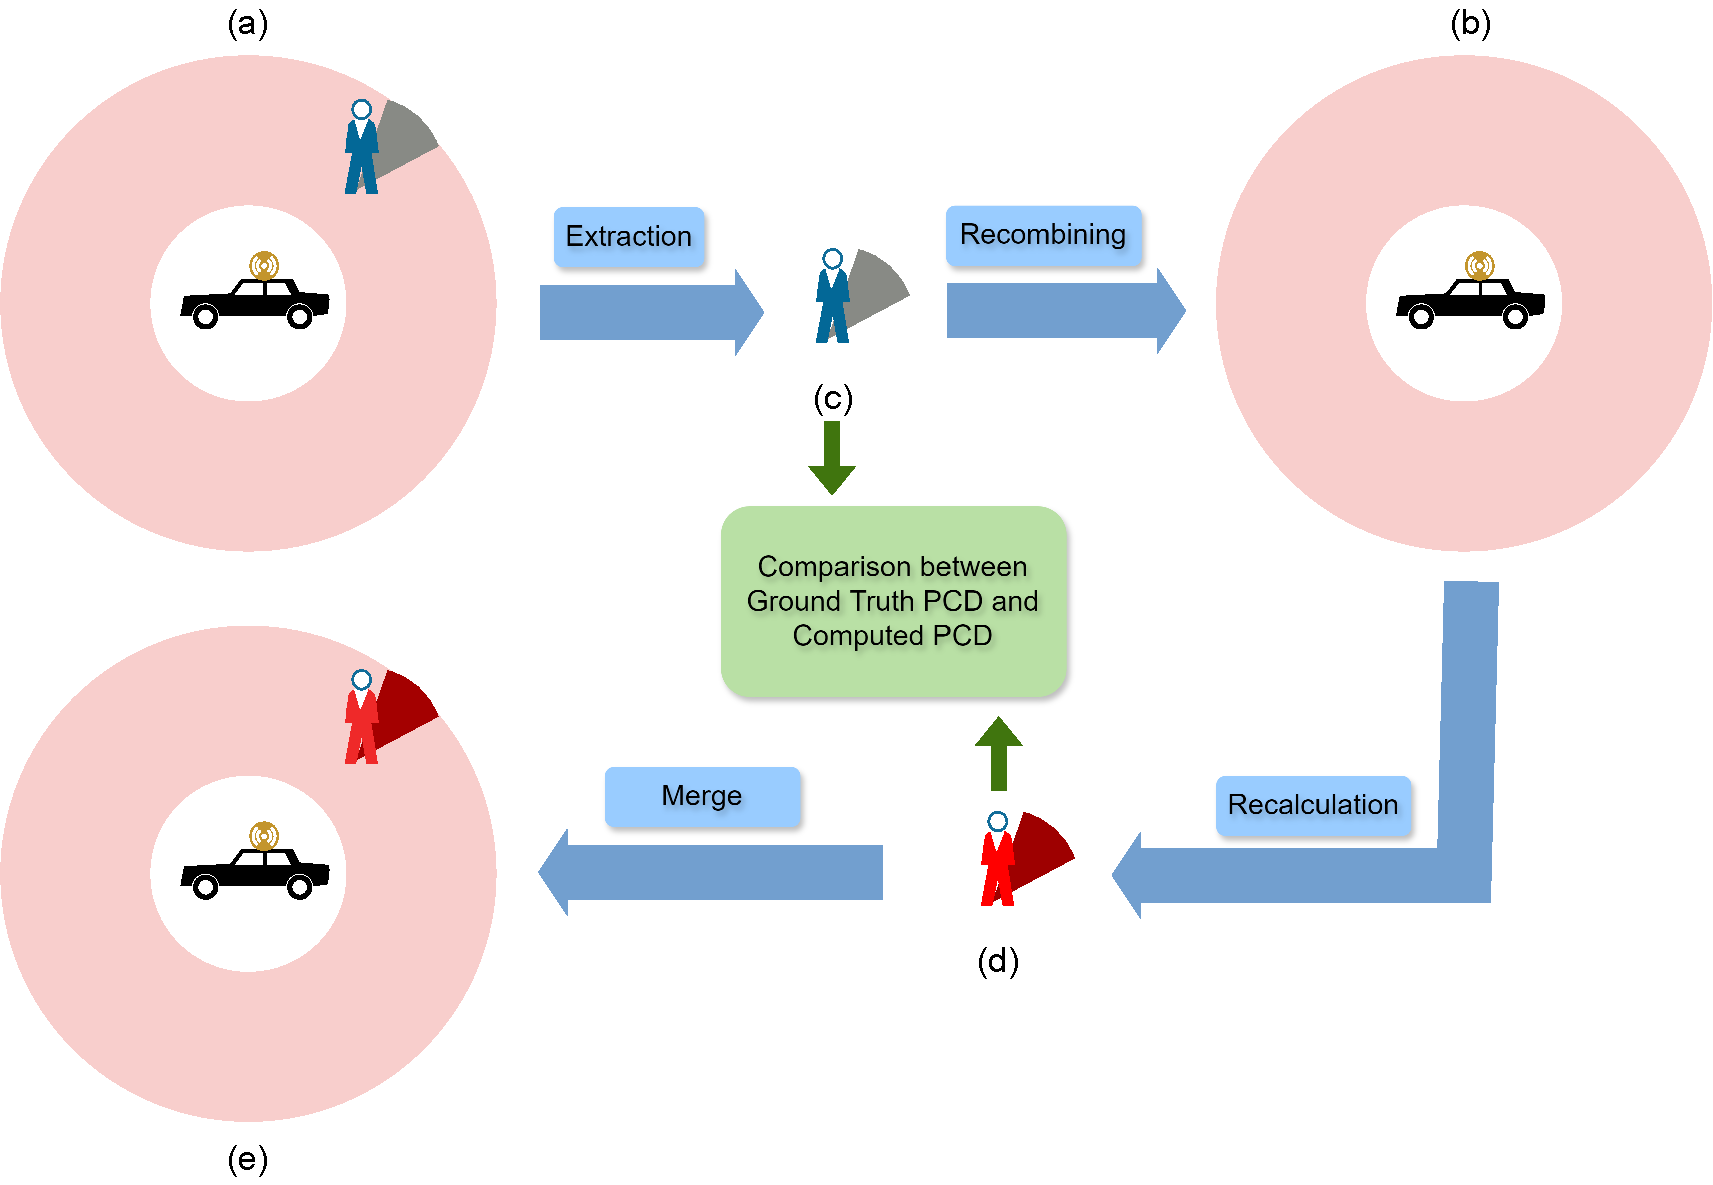
\includegraphics[width=0.75\linewidth]{97_graphics//evaluation/evaluation_step_diagram.pdf}
    \caption[Evaluation Concept Diagram.]{Evaluation Concept Diagram. (a) and (b) present two distinct point clouds featuring equivalent background contexts, with the sole disparity being the presence or absence of a Prototype (person) and its cast shadow. (c) showcases the isolated point cloud representing the Prototype (Original Prototype) and the ground truth shadow. (d) displays the computed point cloud of the person(raycasted point cloud) along with its newly projected shadow (anticipated shadow) onto the Target Scene \acrshort{pcd} \acrshort{roi}(b). (e) Augmented Target Scene Point Cloud.} 
    \label{fig:evaluation-evaluation_step_diagram}
\end{figure}

 The assessment of the thesis output involves a comparative analysis between the point clouds represented in figure \ref{fig:evaluation-evaluation_step_diagram} \((c)\) and \ref{fig:evaluation-evaluation_step_diagram} \((d)\). Figure \ref{fig:evaluation-evaluation_step_diagram} \((c)\) represents the ground truth point cloud of the prototype (person or original prototype) and the shadow projected by the prototype. It is obtained by extracting the desired ground truth point clouds from the source scene point cloud \((a)\). \((d)\) represents the prototype point cloud generated through raycasting (raycasted point cloud of prototype), accompanied by the shadow projected by this new prototype point cloud on the target scene \((b)\). This output encapsulates the culmination of the thesis work.
\((e)\) represents the final augmented target scene point cloud. The source scene point cloud \((a)\) and the target scene cloud \((b)\) are acquired from \acrshort{carla}.

\begin{figure}[htbp]
    \centering
    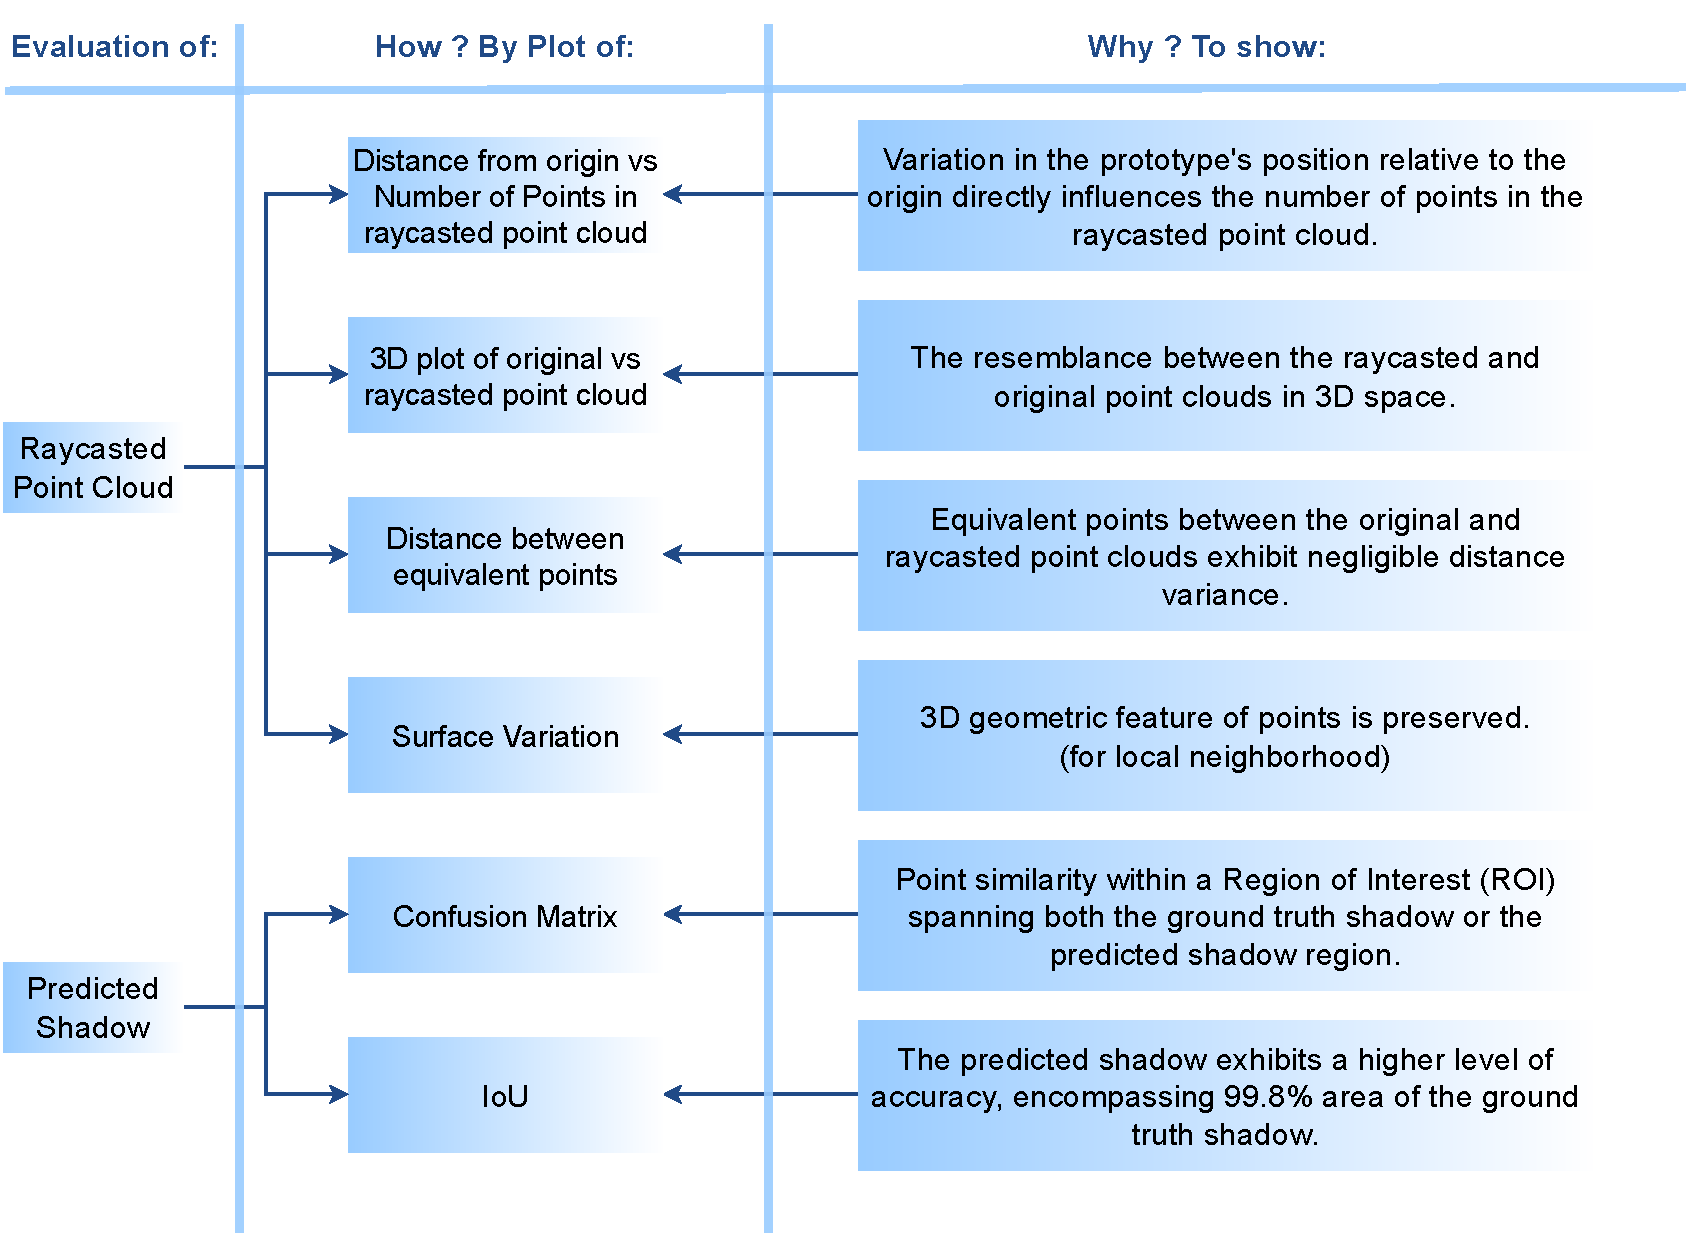
\includegraphics[width=1\linewidth]{97_graphics//evaluation/evaluation_block_diagram.pdf}
    \caption{Evaluation Overview.}
    \label{fig:evaluation-evaluation_block_diagram}
\end{figure}

As outlined in figure \ref{fig:evaluation-evaluation_block_diagram}, raycasted point cloud is analyzed through four graphical representations. A scatter plot is generated wherein the distance of the prototype (person / original prototype PCD) is varied within the target scene cloud from the origin, and subsequently, the raycasted point cloud is calculated. This analysis demonstrates a correlation between the number of raycasted points on the prototype surface and their proximity to the origin, indicating a decrease in the number of points as the distance from the origin increases. Additionally, a 3D plot comparing the original prototype and the raycasted prototype point cloud is constructed without transforming the prototype location to a different position, facilitating visual differentiation between the two sets of points in the cartesian coordinate system. This is represented visually as a comparison between the point cloud of the prototype (person) represented in figure \ref{fig:evaluation-evaluation_step_diagram} \((c)\) and \ref{fig:evaluation-evaluation_step_diagram} \((d)\). Consistency between the original and raycasted prototype point clouds is affirmed by overlapping points observed in the 3D plot. Furthermore, a graph plotting the distance between corresponding points in the original and raycasted prototype \acrshort{pcd} illustrates minimal distance discrepancies between equivalent points. Geometric feature distribution analysis, conducted using equivalent parameters, further confirms the similarity in local geometric features of points between the original prototype point cloud and the raycasted prototype point cloud.

To assess the precision of the predicted shadow, two distinct point clouds are captured: one containing a person and their casted shadow (referred to as the source scene cloud, represented by figure \ref{fig:evaluation-evaluation_step_diagram} \((a)\)), and another identical point cloud lacking the person or their shadow but maintaining similar background information (termed the target scene cloud, represented by figure \ref{fig:evaluation-evaluation_step_diagram} \((b)\)). A prototype (person) point cloud is extracted from the source scene cloud and seamlessly inserted into the target scene cloud without any transformation. Subsequently, the shadow cast by the prototype on the target scene cloud is computed. This is visually depicted as a comparison between the ground truth shadow (the shadow projected by the prototype as shown in figure \ref{fig:evaluation-evaluation_step_diagram} \((c)\) ) and the predicted shadow (the computed shadow of the raycasted prototype as shown in figure \ref{fig:evaluation-evaluation_step_diagram} \((d)\)).

The correctness of the predicted shadow is observed by plotting the confusion matrix and by computing the \acrshort{iou} score as outlined in figure \ref{fig:evaluation-evaluation_block_diagram}. A confusion matrix is constructed, wherein equivalent points between the two point clouds are identified within a \acrfull{roi} using nearest neighbor search. The confusion matrix reveals a high degree of similarity between corresponding points in the selected ROI of both point clouds. Additionally, a plot demonstrating the distance between points in the \acrshort{roi} of the predicted shadow cloud and their equivalents in the original shadow cloud further validates the accuracy of the confusion matrix. \acrfull{iou} between the predicted shadow and the ground truth shadow region is calculated, confirming the precise prediction of the shadow cast by the prototype. The discrepancy in the area of the predicted shadow compared to the ground truth shadow is attributed to the larger surface area of the reconstructed surface (triangle mesh of person surface) relative to the original prototype(person).

\section{Evaluation of Raycasted Point Cloud}

A raycasted point cloud is generated by projecting rays from the origin to the surface of the prototype. The prototype surface is obtained through surface reconstruction into a triangular mesh. Methods like calculation of average distance, comparing the number of points, and comparing the vanilla 3D points were used for the evaluation of raycasted point cloud. These methods are discussed below.
\subsection{Average distance from the Origin vs Number of Points}
With this step, we check the variation of the number of points in the raycasted point cloud when changing the position of the prototype before raycasting concerning origin. The distance between the prototype \acrshort{pcd} and the origin of the target scene \acrshort{pcd} was changed by transforming the extracted prototype to a different location on the target scene \acrshort{pcd}. The distance from a prototype to the origin is calculated by calculating the Euclidean distance from the origin to each point in the prototype \acrshort{pcd}. The average was obtained after dividing the sum of the distances of each point in the prototype \acrshort{pcd} by the number of points. Rays were cast to the surface of the prototype after surface reconstruction.  Change in points number based on different locations of the transformed prototype on the target scene \acrshort{pcd} is observed.

\begin{figure}[htbp]
    \centering
    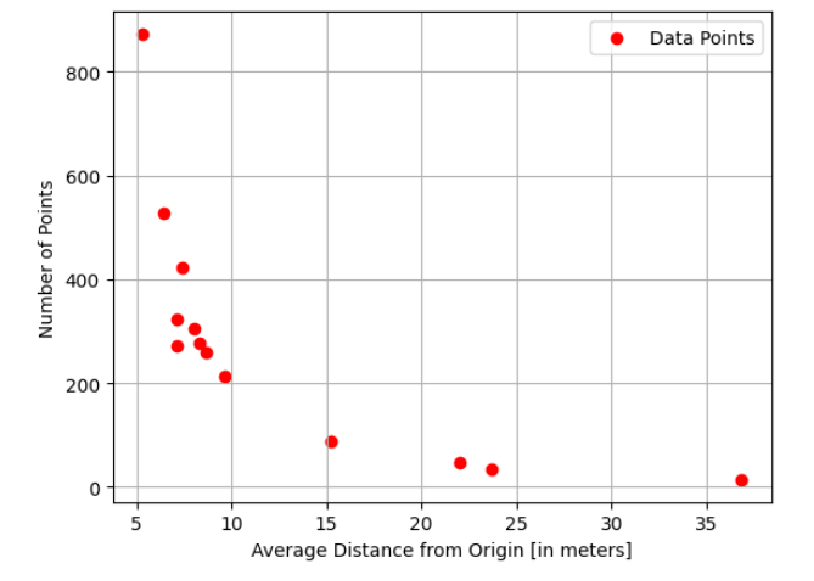
\includegraphics[width=0.8\linewidth]{97_graphics/evaluation/avg_distn_vs_points_numbers.pdf}
    \caption{Averge distance of Prototype (Person) \acrshort{pcd} from the Origin [in meters] vs Number of Points in Raycasted \acrshort{pcd}.}
    \label{fig:evalution_avg_distn_vs_points_number}
\end{figure}
In this figure \ref{fig:evalution_avg_distn_vs_points_number}, the original prototype is positioned at about 7 meters from the origin. The prototype was moved closer toward the origin and farther away from the origin of the target scene \acrshort{pcd}, and the raycasted \acrshort{pcd} of the prototype was calculated. From the graph, as shown in figure \ref{fig:evalution_avg_distn_vs_points_number}, it can be seen that the number of points on the raycasted prototype decreases after an increase in the average distance between the prototype and the origin (more than 7 meters distance). The number of points of the raycasted prototype \acrshort{pcd} increases when the prototype is transformed closer to the origin (less than 7 meters distance).

\subsection{3D plot of the "Original" Prototype and Raycasted Prototype PCD}\label{sec:3dplot}
To visualize the similarities between the corresponding points on the original and raycasted prototype point cloud, a simple 3D plot in the XYZ axis can be analyzed. For this evaluation, the difference between the original prototype and the raycasted prototype is shown where the raycasting was done without transforming the position of the prototype \acrshort{pcd} on the target scene cloud.

\begin{figure}[htbp]
    \centering
    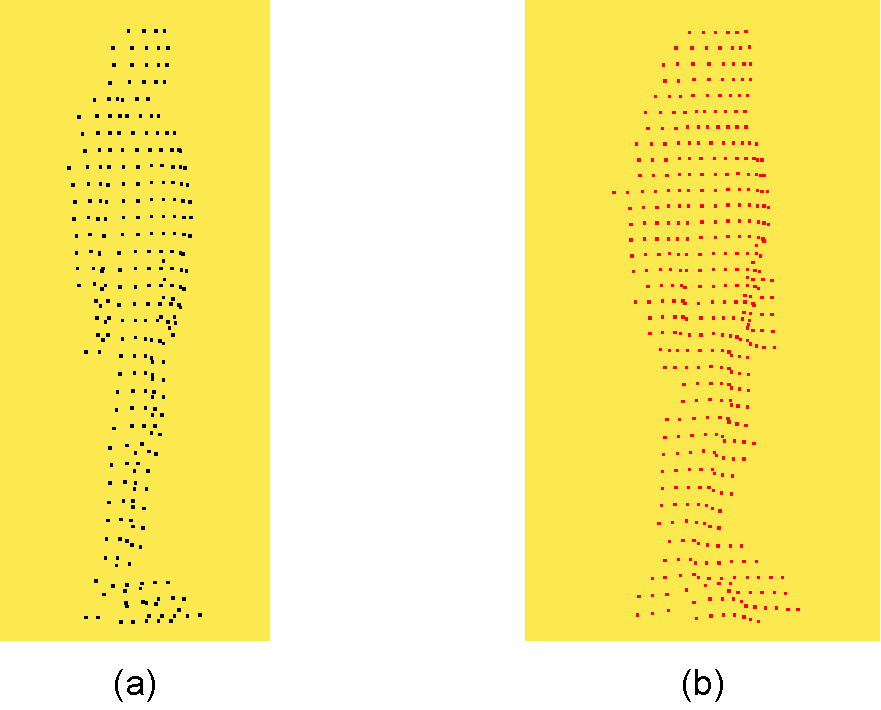
\includegraphics[width=0.75\linewidth]{97_graphics//evaluation/original_vs_raycasted_pcd.pdf}
    \caption[Visualization of Point Clouds.]{Visualization of Point Clouds (a) Original Prototype \acrshort{pcd} (b) Raycasted \acrshort{pcd} of Prototype.}
    \label{fig:evaluation-original_vs_raycasted_pcd}
\end{figure}

Figure \ref{fig:evaluation-original_vs_raycasted_pcd} \((a)\) shows the point cloud of the prototype (person) before raycasting (by the black color points). \((b)\) shows the point cloud of the prototype evaluated after raycasting  (by the red color points). The raycasted point cloud in figure \ref{fig:evaluation-original_vs_raycasted_pcd} \((b)\) is computed without transforming the orientation of the prototype to compare the difference in corresponding points between the two \acrshort{pcd}. Symbolically, it is depicted through the comparison between figure \ref{fig:evaluation-evaluation_step_diagram} \((c)\) and \ref{fig:evaluation-evaluation_step_diagram} \((d)\).

\begin{figure}[htbp]
    \centering
    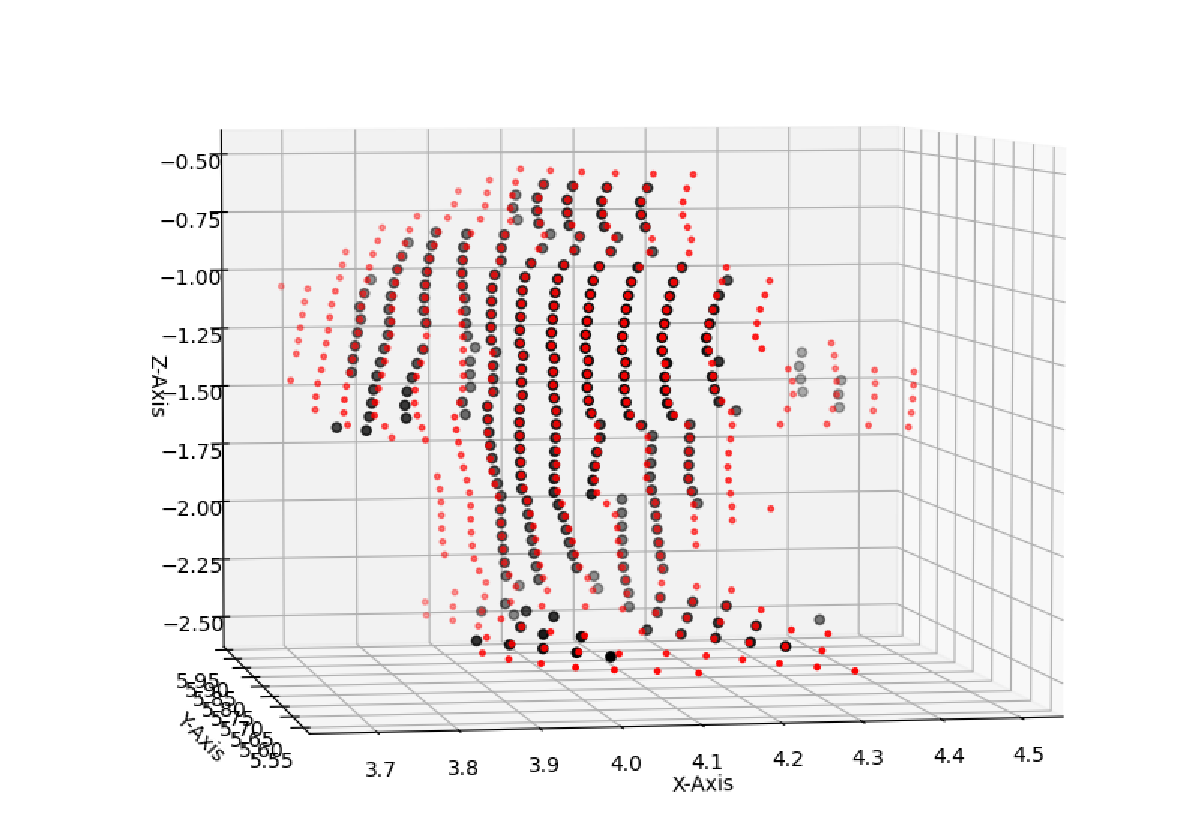
\includegraphics[width=0.8\linewidth]{97_graphics/evaluation/3dxyz_plot.pdf}
    \caption{3D XYZ Plot of Original Prototype \acrshort{pcd} (black) vs Raycasted Prototype \acrshort{pcd} (red).}
    \label{fig:evaluation_3dplot}
\end{figure}

The graph can be viewed in figure \ref{fig:evaluation_3dplot}. The black points in the graph correspond to the point in the prototype before raycasting (representing the \acrshort{pcd} shown in figure \ref{fig:evaluation-original_vs_raycasted_pcd} \((a)\) ). The red points in the graph correspond to the point of the prototype after raycasting (representing the \acrshort{pcd} shown in figure \ref{fig:evaluation-original_vs_raycasted_pcd} \((b)\) ). It can be observed that most of the red points overlap the black points in space, which proves that there is a low difference between the original prototype \acrshort{pcd} and the prototype \acrshort{pcd} after raycasting. Most of the red points that do not overlap with the black points are due to the bigger area of the reconstructed surface of the prototype. Proper filtering of the reconstructed surface triangle mesh could result in the removal of the red outliers.

\subsection{Distance between the "Equivalent" Points in the "Original" Prototype and Raycasted Prototype PCD}
Distance between the corresponding points was calculated between the original prototype \acrshort{pcd} and the prototype \acrshort{pcd} after raycasting. The raycasting was performed on the original prototype surface without transformation. We calculated the average distance between the black points and the corresponding red points of figure \ref{fig:evaluation_3dplot}. To find the equivalent points between two clouds, the nearest neighbor points between the two \acrshort{pcd} is computed. Spheres with different values of radius were experimented with for the calculation of the nearest neighbor. Neighbors for a point in the original prototype \acrshort{pcd} were calculated from the raycasted \acrshort{pcd} that falls within the radius of the sphere, centered around the ego point. The neighbor that has the minimum distance from the ego point is chosen. This point in the raycasted prototype \acrshort{pcd} is considered the equivalent point of the ego point in the original prototype \acrshort{pcd}. Sphere size can be lower or higher for neighbor search. This is because whatever the size of the sphere, we are extracting a point from the neighborhood inside the sphere that has the least distance from the ego point or center of the sphere. However, too low value for radius might lead to not finding any neighbors.
\begin{figure}[htbp]
    \centering
    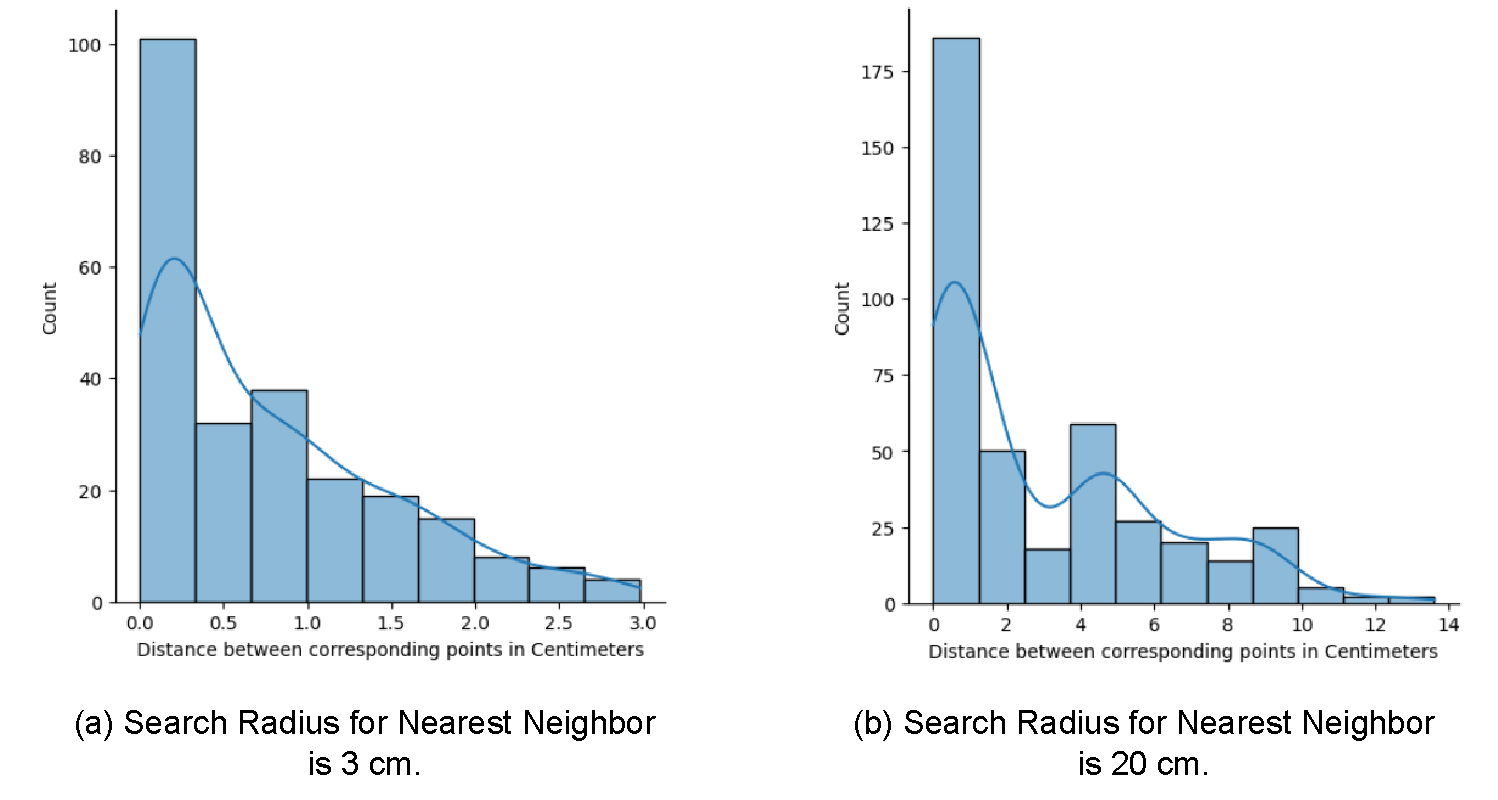
\includegraphics[width=1\linewidth]{97_graphics/evaluation/distn_betn_corresponding_points_in_raycasting.pdf}
    \caption{Distance (in centimeters) between the "equivalent" points in the Prototype(Original) and Raycasted Prototype \acrshort{pcd}.}
    \label{fig:evaluation_distn_corresponding_points}
\end{figure}

Figure \ref{fig:evaluation_distn_corresponding_points} shows plots of the distance between the black points and their equivalent red points from figure \ref{fig:evaluation_3dplot}. Figure (a) is plotted after finding the nearest neighbor with a search within the sphere of radius 3 cm centered around an ego point. When searching the neighbor with a sphere of radius 3cm, out of 408 points in the raycasted \acrshort{pcd}, 163 number of equivalent points were not found in the original \acrshort{pcd}. Using a higher radius value for neighbor search (20 cm), all the points in the red points were found to have their equivalent black points. This is shown by part (b) of the figure. The figure shows that a high concentration of equivalent points is situated within 0-3 cm distance apart from eachother.

\subsection{Surface Variation Plot}
Surface variation for the point cloud represented by red points and black points in figure \ref{fig:evaluation_3dplot} was calculated and plotted.

\begin{figure}[htbp]
    \centering
    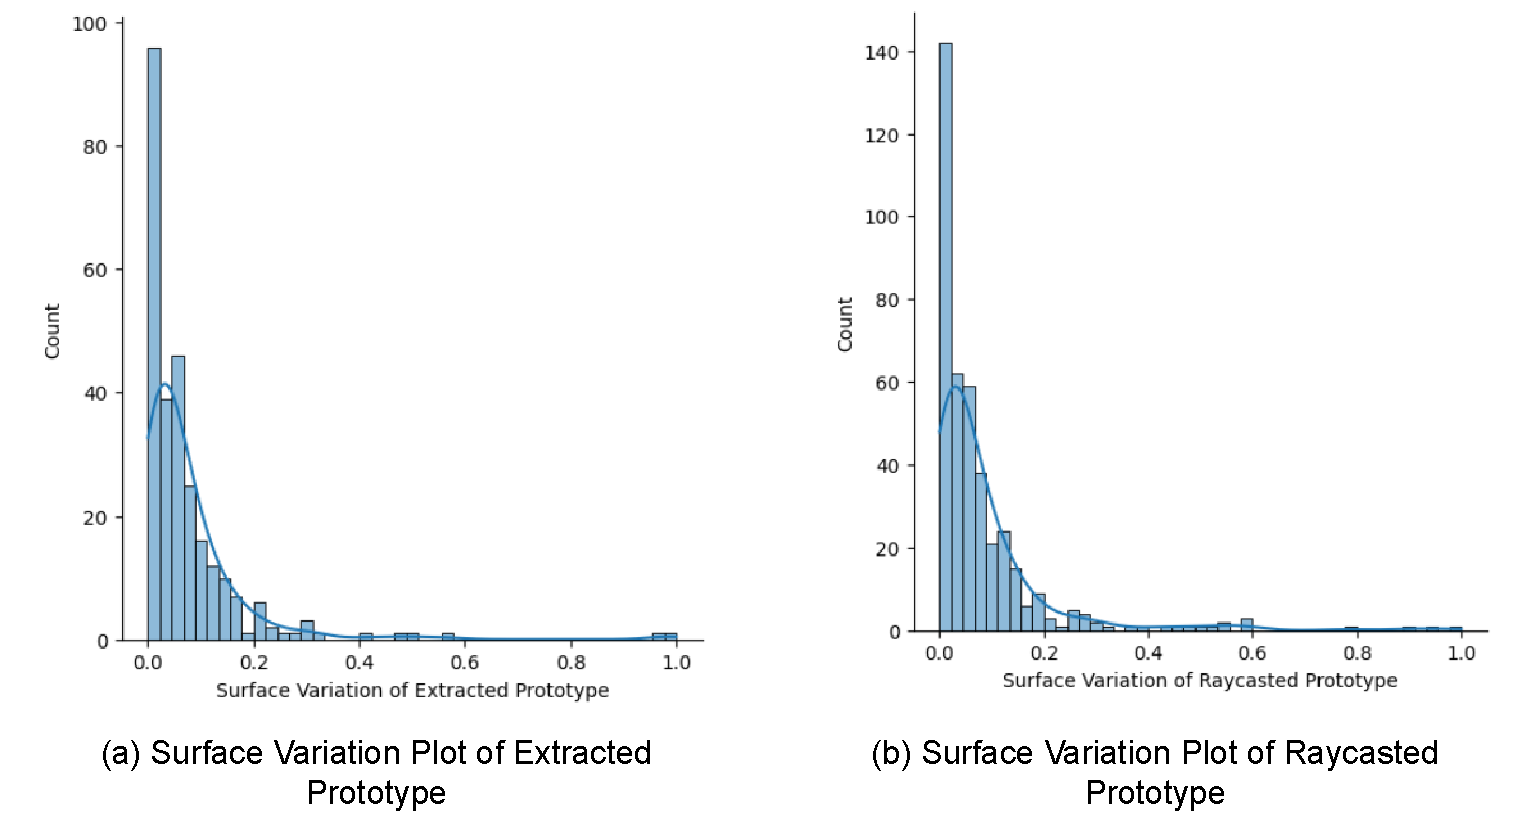
\includegraphics[width=1\linewidth]{97_graphics/evaluation/sv_plots.pdf}
    \caption{Surface Variation Plot between the Extracted (Original) Prototype and Raycasted Prototype \acrshort{pcd}.}
    \label{fig:evaluation-sv_plots}
\end{figure}

For this experiment, a radius of 30cm with a maximum value of the nearest neighbor was taken to be 6 as a parameter to calculate the nearest neighbor using KDTree in open3d. Using the formula for surface variation as described in equation \ref{eq:surf_var}, surface variation for each point in the \acrshort{pcd} is calculated. The obtained result is normalized on a scale of 0 to 1 and the corresponding plot is displayed as shown in figure \ref{fig:evaluation-sv_plots}. The figure shows the similarities in local geometric features (surface variation ) of points between the two point clouds.


\section{Evaluation of Casted Shadow}
For the evaluation purpose, point cloud representing a "flat" surface was captured from the \acrshort{carla}. This point cloud represents a target scene where we would like to do a shadow casting. A prototype "person" was spawned in some location in the target region without changing the orientation of the lidar sensor and the point cloud was saved. This point cloud corresponds to the source scene \acrshort{pcd}. The prototype \acrshort{pcd} is extracted from the source scene cloud and placed in the target scene \acrshort{pcd}. Shadow casting by the prototype is performed on the target scene \acrshort{pcd} and the final augmented point cloud is saved. The prototype \acrshort{pcd} of the person is not transformed in the target scene. The difference between the target scene cloud and the source scene cloud is the availability of the person and its casted shadow, the rest of the points are similar in both point clouds, i.e. background information is similar on both point clouds. 
Figuratively, it is illustrated by assessing the person's cast shadow in figure \ref{fig:evaluation-evaluation_step_diagram} \((c)\) and \ref{fig:evaluation-evaluation_step_diagram} \((d)\).
A region is selected from the source scene cloud which constitutes of shadow projected by the prototype. This region is the ground truth shadow region as shown in figure \ref{fig:evaluation-shadow_difference_roi} \((a)\). The corresponding region is selected on the target scene cloud where the raycasted point cloud of the prototype is computed and the shadow projected by the new prototype point cloud is calculated. This region is the predicted shadow region as shown in figure \ref{fig:evaluation-shadow_difference_roi} \((b)\).
\begin{figure}[htbp]
    \centering
    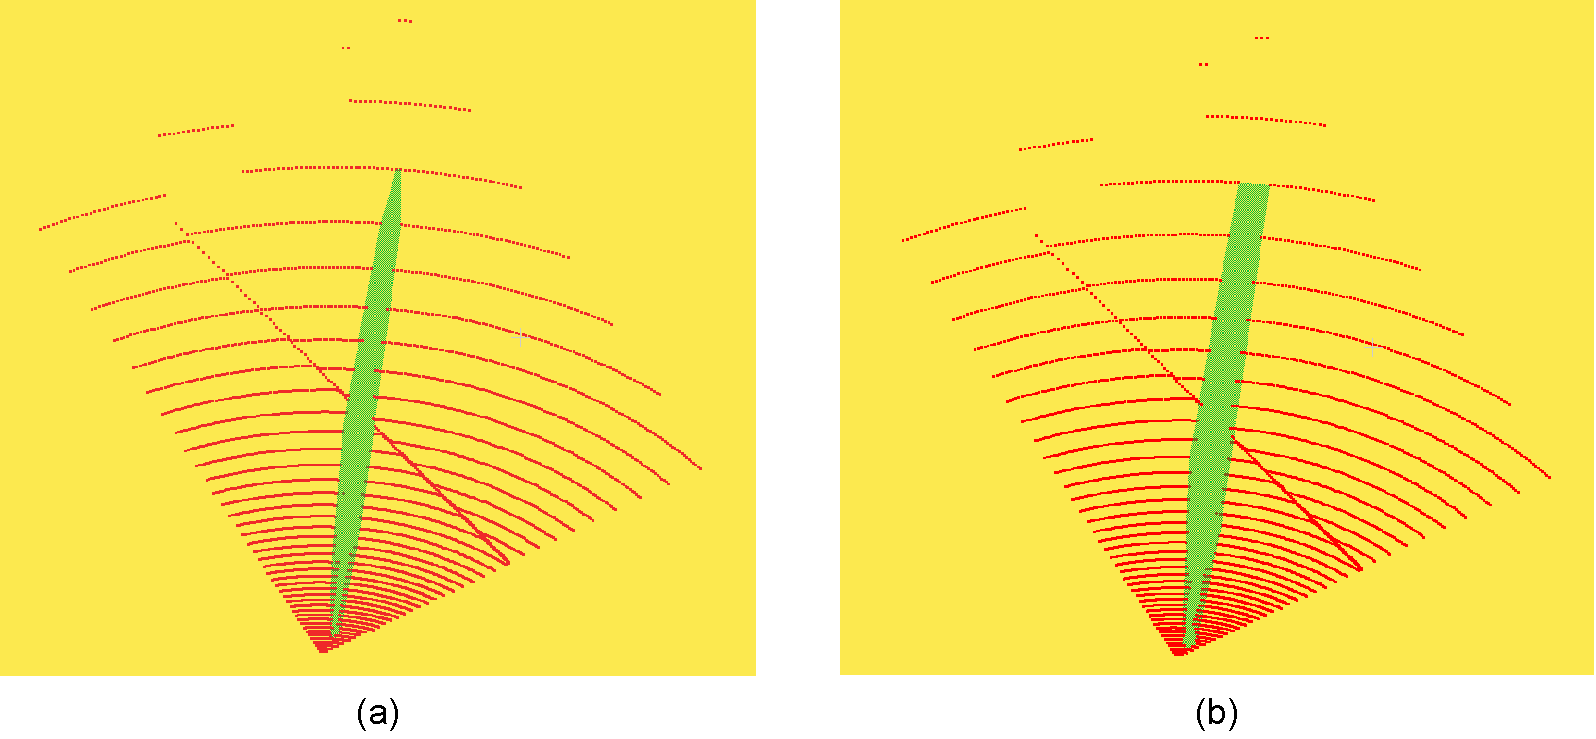
\includegraphics[width=1\linewidth]{97_graphics//evaluation/shadow_difference_roi.pdf}
    \caption[Shadow Casted by the Prototype.]{Shadow Casted by the Prototype (person) \acrshort{pcd} on a \acrshort{roi}, represented by green color region (a) Ground Truth Shadow (b) Predicted Shadow.}
    \label{fig:evaluation-shadow_difference_roi}
\end{figure}

Figure \ref{fig:evaluation-shadow_difference_roi} shows the shadow projected by the prototype. The green-colored region on both \((a)\) and \((b)\) represents the approximate shadow projected by the prototype. \((a)\) represents ground truth shadow region and \((b)\) represents predicted shadow region.  Shadow is calculated and computed for only a selected region on the target scene cloud. The selected \acrfull{roi} is shown by the red color point in figure \ref{fig:evaluation-shadow_difference_roi}.

\subsection{Confusion Matrix}
Comparison between the shadow is done by finding the corresponding points in \acrshort{roi} where the ground truth shadow and the anticipated shadow is projected, i.e. between points in figure \ref{fig:evaluation-shadow_difference_roi} \((a)\) and \((b)\). The nearest neighbor search was done to find the equivalent points in the selected \acrshort{roi} of the ground truth shadow and anticipated shadow cloud. The radius of the sphere for the neighbor search was taken to be 3 centimeters. If no neighbors were found on the corresponding point cloud within this region, the point was considered to be not found. From the found neighbors, based on some threshold value, the neighbors were filtered. If there exists a neighbor after filtering with some threshold distance, the point was considered to be found on both point clouds. If not, the point was labeled as not found. A confusion matrix is plotted as shown in figure \ref{fig:evaluation_cm}.

\begin{figure}[htbp]
    \centering
    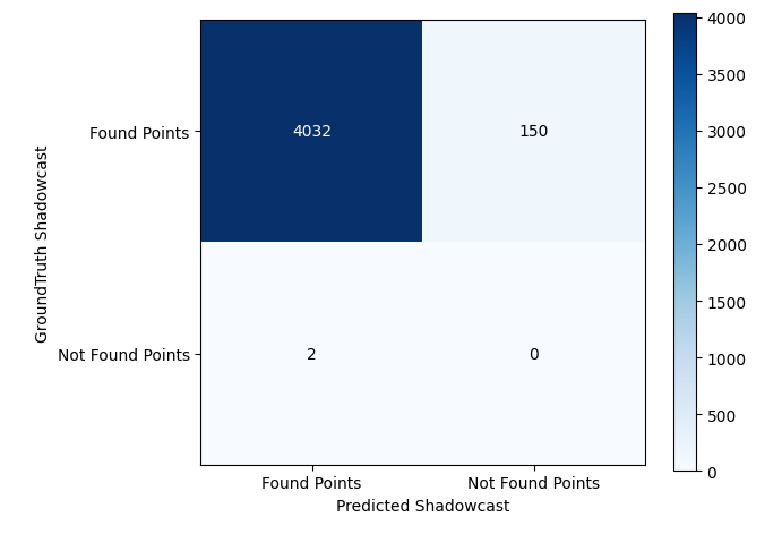
\includegraphics[width=1\linewidth]{97_graphics/evaluation/cm_shadowcast.pdf}
    \caption{Confusion matrix.}
    \label{fig:evaluation_cm}
\end{figure}

Some observations can be made from the confusion matrix in figure \ref{fig:evaluation_cm}. Equivalent points for 150 points from the \acrshort{roi} containing the ground truth shadow were not found in the \acrshort{roi} containing the predicted shadow region, i.e between \ref{fig:evaluation-shadow_difference_roi} \((a)\) and \ref{fig:evaluation-shadow_difference_roi} \((b)\). 2 points available on the ROI containing predicted shadow \acrshort{pcd} were not found in the ROI containing the ground truth shadow region. 4032 corresponding points were found in both regions. Unable to say about the points not found on both, the true negative section in the confusion matrix is labeled as 0. From the confusion matrix and using equations \ref{eq:accuracy}, \ref{eq:precision}, \ref{eq:recall}, and \ref{eq:f1-score}, the following metrics are observed as shown in table \ref{tab:evaluation-conf_matrix}. 

\begin{table}[htbp]
    \centering
    \renewcommand{\arraystretch}{1.5} % Adjust vertical spacing
    \setlength{\tabcolsep}{10pt} % Adjust horizontal spacing
    
    \begin{tabular}{|>{\centering\arraybackslash}m{4cm}|>{\centering\arraybackslash}m{3cm}|} % Adjust column width and alignment
        \hline
        \textbf{Metrics} & \textbf{Value} \\
        \hline
        True Positive & 4032 \\
        \hline
        True Negative & 0 \\
        \hline
        False Positive & 2 \\
        \hline
        False Negative & 150 \\
        \hline
        Accuracy & 0.963 \\
        \hline
        Precision & 0.999 \\
        \hline
        Recall & 0.964 \\
        \hline
        F1-Score & 0.981 \\
        \hline
    \end{tabular}
    \vspace{10pt}
    \caption{Performance Metrics Calculated for ROI containing \acrshort{gt} Shadow Region and Predicted Shadow Region.}
    \label{tab:evaluation-conf_matrix}
\end{table}

The calculation proves that the shadow projection has a high accuracy and a very low error rate.

\begin{figure}[htbp]
    \centering
    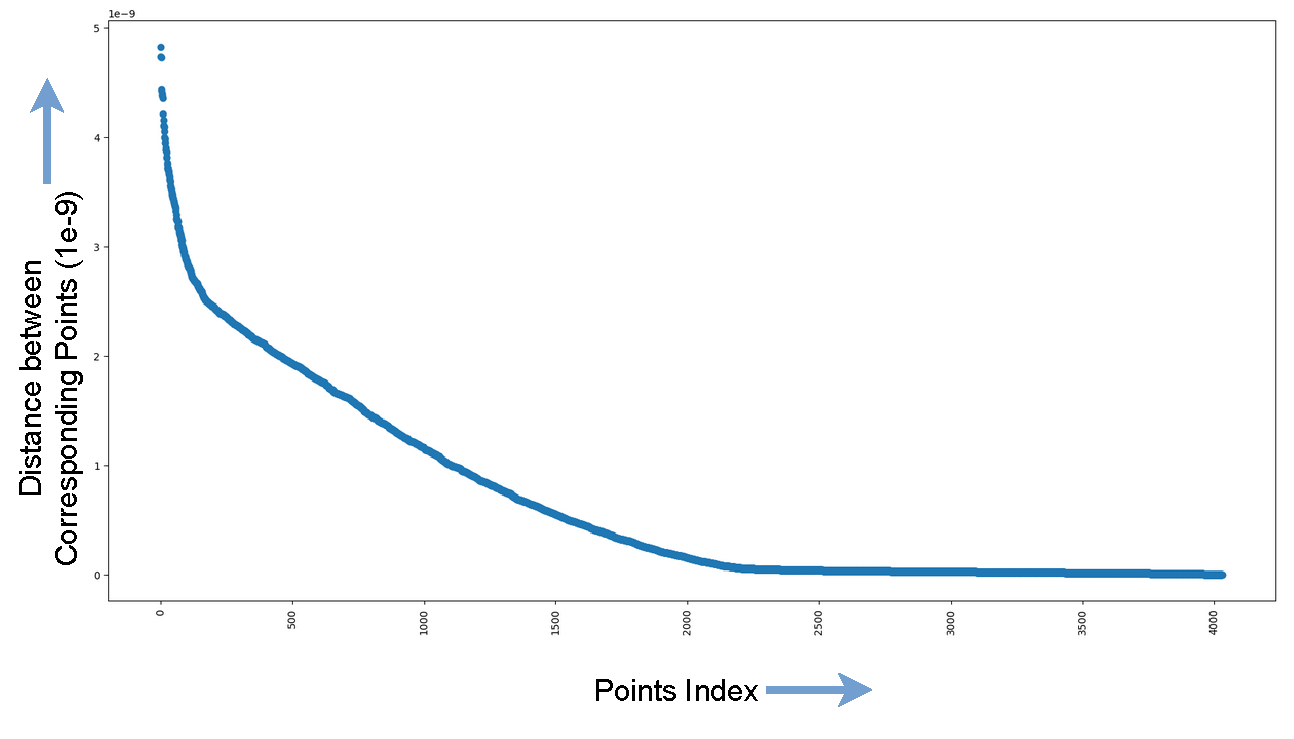
\includegraphics[width=0.7\linewidth]{97_graphics//evaluation/distn_betn_corresponding_points_in_shadowcasting.pdf}
    \caption{Distance between corresponding points for selected \acrshort{roi} containing \acrshort{gt} Shadow and Predicted Shadow of Prototype \acrshort{pcd}.}
    \label{fig:evaluation-distn_betn_corresponding_points_in_shadowcasting}
\end{figure}

Figure \ref{fig:evaluation-distn_betn_corresponding_points_in_shadowcasting} shows the distance between the corresponding points in the ROI containing the predicted shadow region and the ground truth shadow region. The figure verifies that the points that were considered to be similar in both regions are very similar as the distance between the equivalent points is in the order of \(10^{-9}\) meters.

\subsection{Intersection over Union}
For the calculation of \acrfull{iou}, the contour points of the shadow region were first extracted for both the point clouds(ground truth shadow and predicted shadow region). The contour points are represented by the boundary points of the green-colored region of figure \ref{fig:evaluation-shadow_difference_roi}. The extracted 3d-points were projected to the XY plane; i.e. by making the z-value of each point zero. The area of the region occupied by the surface bounding the contour points (i.e. the shadow region) was calculated. This is shown approximately by green-colored region in figure \ref{fig:evaluation-shadow_difference_roi}. The absolute region representing the ground truth shadow and predicted shadow is shown in figure \ref{fig:evaluation-shadow_gt_pred}.
\begin{figure}[htbp]
    \centering
    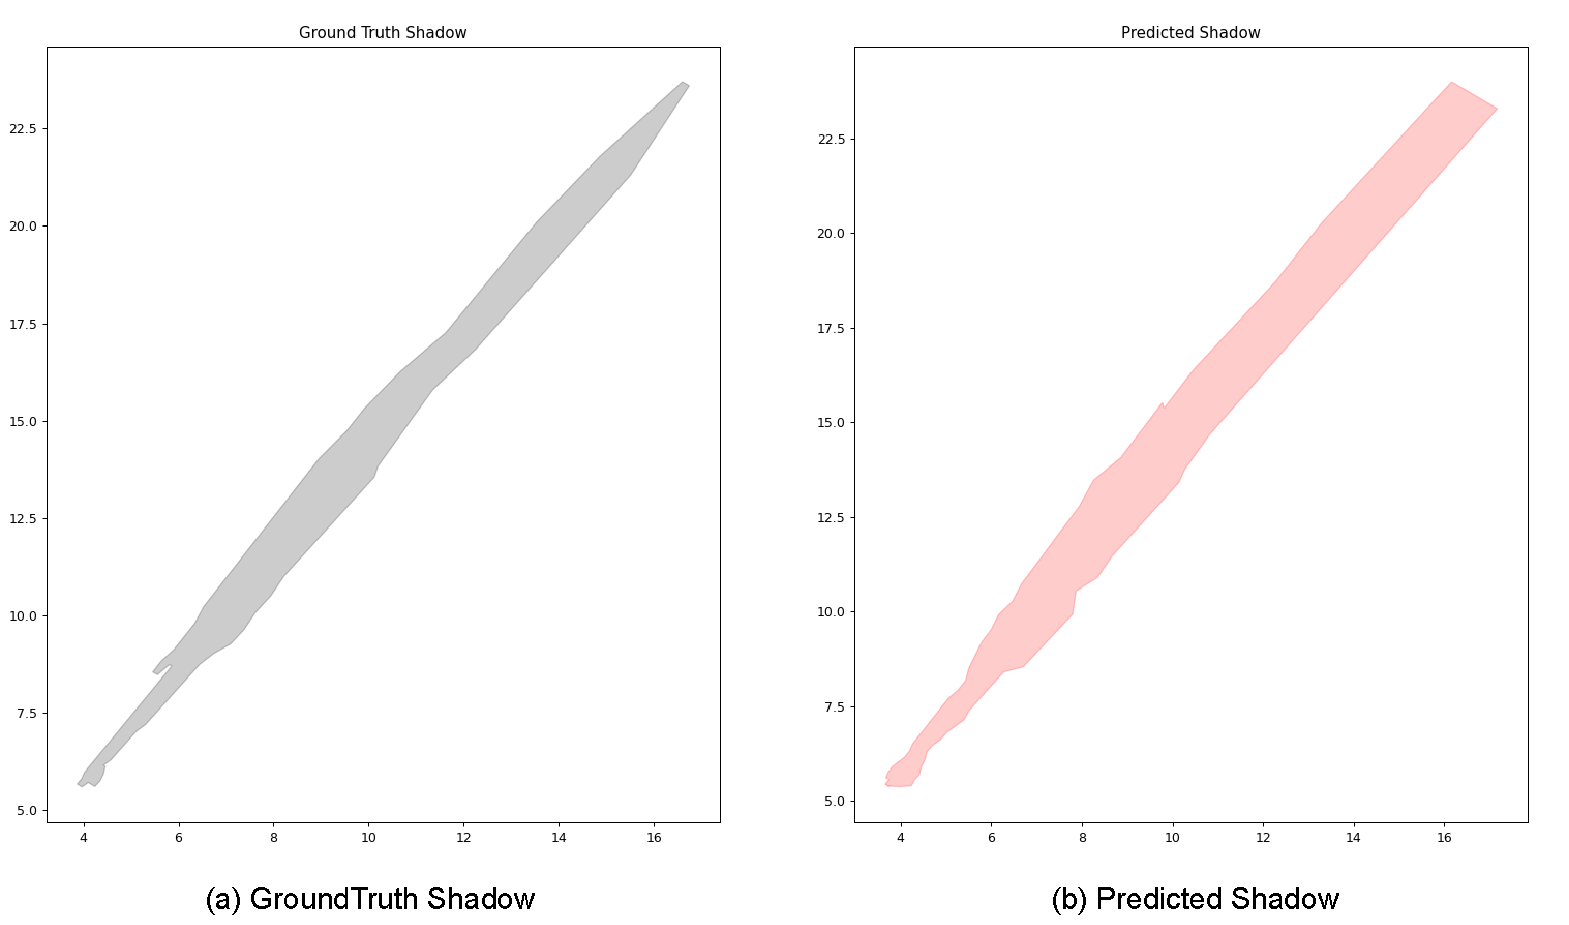
\includegraphics[width=0.7\linewidth]{97_graphics//evaluation/shadow_gt_pred.pdf}
    \caption{Plot of Ground Truth Shadow and Predicted Shadow.}
    \label{fig:evaluation-shadow_gt_pred}
\end{figure}

Figure \ref{fig:evaluation-shadow_iou} (a) shows the intersection region between the ground truth shadow and predicted shadow by green color. (b) shows the union area between the two regions.

\begin{figure}[htbp]
    \centering
    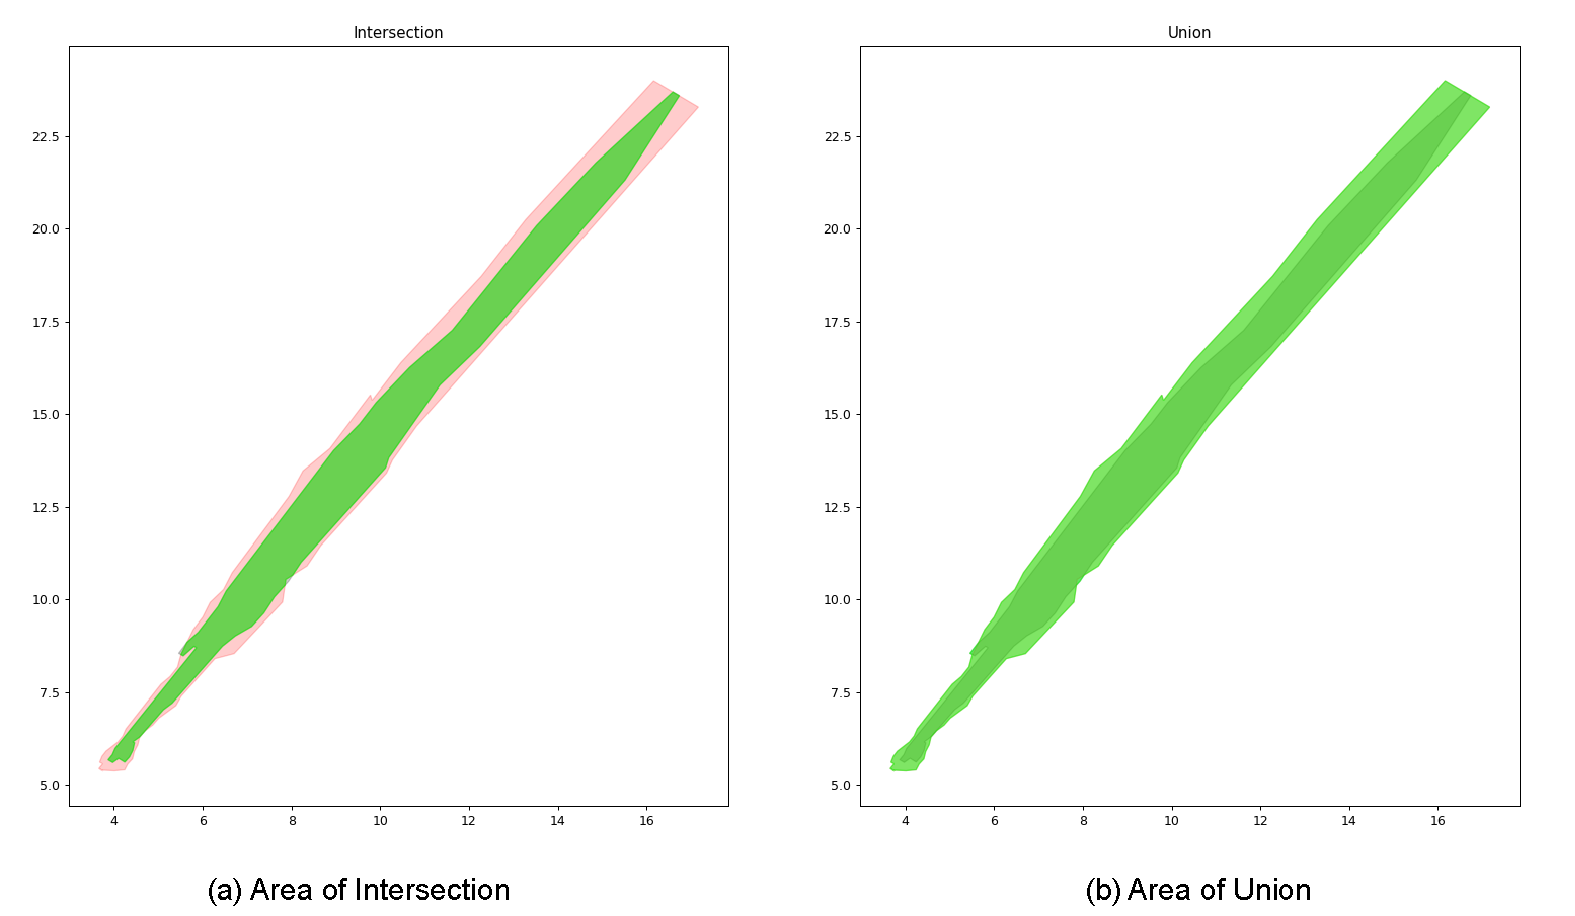
\includegraphics[width=0.7\linewidth]{97_graphics//evaluation/shadow_iou.pdf}
    \caption{Intersection and Union between the \acrshort{gt} Shadow Region and Predicted Shadow Region.}
    \label{fig:evaluation-shadow_iou}
\end{figure}

\begin{equation}\label{eq:gt_shadow_pp}
    PP_{\text{GT}} = \left( \frac{A_{\text{GT}} - A_{\text{GT}\setminus\text{Pred}}}{A_{\text{GT}}} \right) \times 100\%
\end{equation}

Equation \ref{eq:gt_shadow_pp} gives the percentage of \acrshort{gt} shadow accurately predicted from the project. \(PP_{GT}\) represents the Prediction Percentage of GT Shadow that was accurately predicted. \(A_{GT}\) represents the Area of the \acrfull{gt} shadow region. \(A_{\text{GT}\setminus\text{Pred}}\) is the Area in \acrshort{gt} shadow region that is not predicted as the shadow region of Prototype.

Observations can be made as shown in table \ref{tab:evaluation-iou}.

\begin{table}[htbp]
    \centering
    \renewcommand{\arraystretch}{1.5} % Adjust vertical spacing
    \setlength{\tabcolsep}{10pt} % Adjust horizontal spacing
    
    \begin{tabular}{|>{\centering\arraybackslash}m{10cm}|>{\centering\arraybackslash}m{3cm}|} % Adjust column width and alignment
        \hline
        \textbf{Metrics} & \textbf{Value} \\
        \hline
        Area of Ground Truth (GT) Shadow Region & 17.318 m$^2$ \\
        \hline
        Area of Predicted Shadow Region & 25.886 m$^2$\\
        \hline
        Area of Intersection & 17.293 m$^2$ \\
        \hline
        Area of Union & 25.910 m$^2$ \\
        \hline
        Intersection over Union (IoU) & 0.667 \\
        \hline
        Area in Ground Truth Shadow not in Predicted Shadow & 0.0248 m$^2$ \\
        \hline
        Area in Predicted Shadow not in Ground Truth Shadow & 8.592 m$^2$ \\
        \hline
        Percentage of GT Shadow Region accurately Predicted & 99.856 \%  \\
        \hline
    \end{tabular}
    \vspace{10pt}
    \caption{Metrics assessing the Intersection and Union between \acrshort{gt} Shadow Region and Predicted Shadow Region.}
    \label{tab:evaluation-iou}
\end{table}

Using equation \ref{eq:gt_shadow_pp}, it is calculated that about \(99.856 \%\) of the ground truth shadow region was predicted. The IoU score was \(0.667\). It can be improved by filtering the reconstructed surface mesh to represent the prototype accurately.

